\chapter{RESULTS}

\section{Experimental Setup and Evaluation Protocol}
We evaluated the framework on video datasets with varied crowd densities, lighting levels, and obstructions.

\subsection{Test Environments and Datasets}
The evaluation covered four primary clinical and activity scenarios:
\begin{enumerate}[(i)]
    \item \textbf{Scenario A: Hospital OPD Waiting Area (\texttt{fig4}):} A crowded outpatient waiting hall with occupants on wooden benches and dim peripheral light. While young children are generally present in the full unclipped hospital recordings, the selected 700-frame evaluation sequence contained zero children.
    \item \textbf{Scenario B: Hospital Old GF Pharmacy (\texttt{fig5}):} An active hospital dispensary corridor with heavy adult traffic, queues at wooden counters, and patients standing behind adults.
    \item \textbf{Scenario C: Kindergarten Playroom (\texttt{fig2}):} An open play area with rapid child movement, varied body angles, and scale changes.
    \item \textbf{Scenario D: Indoor Activity Zone with Furniture Obstructions (\texttt{fig3}):} An indoor area with heavy physical obstructions ($>70\%$) from furniture obstacles and climbing movement.
\end{enumerate}

\subsection{Rationale for Multi-Environment Evaluation}
Ethically usable pediatric clinical CCTV footage was not required to evaluate every framework component independently. The evaluation therefore separates environmental validity from demographic stress testing. Clinical hospital sequences evaluate the target deployment environment. This environment includes specific camera geometry, lighting, waiting-room layouts, queues, and adult crowd interactions. Kindergarten and domestic playroom sequences provide verified pediatric subjects under varied posture, movement, scale, and occlusion conditions. The combined evaluation tests if the framework remains operational across the clinical imaging environment and these specific pediatric visual conditions. This constitutes a cross-domain feasibility evaluation rather than a claim of complete clinical validation.
\subsection{Quantitative Performance Metrics}
We measure model performance with standard detection and counting metrics:
\begin{align}
    \text{Precision} &= \frac{TP}{TP + FP}, \qquad \text{Recall} = \frac{TP}{TP + FN} \\
    F_1\text{-Score} &= 2 \times \frac{\text{Precision} \times \text{Recall}}{\text{Precision} + \text{Recall}} \\
    \text{MAPE} &= \frac{1}{N}\sum_{k=1}^N \frac{|C_{true}^{(k)} - C_{pred}^{(k)}|}{C_{true}^{(k)}} \times 100\% \\
    \text{Census Accuracy} &= \left( 1 - \frac{\sum_{k=1}^{N}|C^{(k)}_{true} - C^{(k)}_{pred}|}{\sum_{k=1}^{N}C^{(k)}_{true}} \right) \times 100\%
\end{align}
\subsection{Hardware and Execution Environment}
We ran all online benchmark evaluations on a host workstation without discrete GPU acceleration:
\begin{itemize}
    \item \textbf{Processor:} Intel Core i7-10610U CPU @ 1.80 GHz (up to 2.30 GHz base clock, 4 physical cores, 8 execution threads). The processor supports native 256-bit AVX2 vector SIMD instructions and FMA3.
    \item \textbf{System Memory:} 16.0 GB DDR4 RAM (15.8 GB usable memory).
    \item \textbf{Inference Engines:} ONNX Runtime 1.29.0 with native \texttt{CPUExecutionProvider}, Intel OpenVINO 2026.3, and PyTorch 2.14.0+cpu.
\end{itemize}
Offline teacher training used an NVIDIA RTX GPU testbed, as described in Section \ref{sec:distill_bench}.

\subsection{Base Model and Fine-Tuned Classifier Evaluation}
The Stage 1 detector uses the off-the-shelf YOLO26s architecture. This base model combines a CSPDarknet feature backbone with decoupled anchor-free detection heads (9.6 million parameters). It operates solely to detect generic human shapes.

For Stage 2, we fine-tuned a custom demographic classifier (\texttt{Pediatric-Model-ONNX}). We trained this model using a unified dataset consisting of 2,413 images (2,342 successfully labeled) containing 3,757 annotations of indoor and outdoor scenes featuring children and adults. We partitioned the data by unique video sequence into 70\% training (1,689 images), 15\% validation (362 images), and 15\% testing (362 images). This strict sequence-level separation prevents identical individuals (same clothing, background, lighting) from appearing in both training and test sets.

Training used the Stochastic Gradient Descent (SGD) optimizer with momentum 0.937, weight decay 0.0005, and initial learning rate $\eta_0 = 0.01$ with cosine decay to $0.0001$. The model trained for 100 epochs with batch size 16.

Table \ref{tab:detector_benchmark} compares the baseline off-the-shelf detector with the proposed multi-stage pipeline on the pediatric test data.

\begin{table}[htbp]
\centering
\caption{Detection Performance Comparison of Base YOLO26s vs.\ Proposed Multi-Stage Pipeline}
\label{tab:detector_benchmark}
\resizebox{\columnwidth}{!}{%
\begin{tabular}{lcccccc}
\toprule
\textbf{Model Configuration} & \textbf{Input Res.} & \textbf{Params} & \textbf{mAP@50} & \textbf{mAP@[50:95]} & \textbf{Heavy Occ. mAP} & \textbf{CPU FPS} \\
\midrule
Base YOLO26s (Pretrained) & $640 \times 640$ & 9.6M & 53.4\% & 36.9\% & 0.1\% & 36.4 \\
Proposed Multi-Stage Pipeline & $640 \times 640$ & 11.7M & \textbf{67.1\%} & \textbf{43.7\%} & \textbf{0.5\%} & 8.1 \\
\bottomrule
\end{tabular}%
}
\end{table}

The decoupled multi-stage approach increased demographic mAP@50 by $13.7\%$ absolute points (from $53.4\%$ to $67.1\%$) compared to using the off-the-shelf generic baseline model for classification.

\section{Distillation Exploratory Benchmark vs.\ Proposed Architecture}\label{sec:distill_bench}
Table \ref{tab:distill_comparison} compares the exploratory Knowledge Distillation (KD) models, the baseline detector, and our multi-stage architecture.

\begin{table}[htbp]
\centering
\caption{Comparative Evaluation of Exploratory Distillation vs.\ Proposed Multi-Stage Pipeline}
\label{tab:distill_comparison}
\resizebox{\textwidth}{!}{%
\begin{tabular}{lccccc}
\toprule
\textbf{Architecture / Model} & \textbf{Precision} & \textbf{Recall} & \textbf{$F_1$-Score} & \textbf{Census MAPE} & \textbf{Throughput (FPS)} \\
\midrule
Teacher: YOLOv8x-CDD & 0.842 & 0.791 & 0.816 & 18.4\% & 8.2 (GPU) \\
Student: Distilled YOLOv8n & 0.765 & 0.710 & 0.736 & 26.2\% & 32.1 (CPU) \\
Baseline: YOLO26s (Direct) & 0.884 & 0.832 & 0.857 & 14.1\% & 36.4 (CPU) \\
\textbf{Proposed: Multi-Stage Framework} & \textbf{0.991} & \textbf{0.985} & \textbf{0.988} & \textbf{0.0\%} & \textbf{8.1 (CPU)} \\
\bottomrule
\end{tabular}%
}
\vspace{0.15cm}
\parbox{\textwidth}{\footnotesize \textit{Note:} Teacher model pre-training was evaluated offline on an NVIDIA RTX GPU testbed (8.2 FPS). All other models and the proposed multi-stage pipeline execute on host CPU hardware.}
\end{table}

The distilled student model achieved lower accuracy ($F_1 = 0.736$, $\text{MAPE} = 26.2\%$). This outcome may not stem solely from architectural failure. Annotation noise and poor data quality may have contributed. The training data lacked sufficient steep CCTV angles and dense crowding examples. The distillation algorithm faithfully transferred features from the teacher, but those features lacked reliable pattern recognition for distant or partially visible toddlers. These data limitations prompted the shift to a decoupled multi-stage architecture. This architecture separates spatial detection from demographic classification.

\subsection{Component Ablation Analysis}
Table \ref{tab:component_ablation} reports incremental ablation results across the pipeline modules.

\begin{table}[htbp]
\centering
\caption{Cumulative Component Addition Study on the Standardized Evaluation Corpus}
\label{tab:component_ablation}
\resizebox{\textwidth}{!}{%
\begin{tabular}{lccccc}
\toprule
\textbf{Pipeline Configuration} & \textbf{Precision} & \textbf{Recall} & \textbf{$F_1$-Score} & \textbf{Census MAPE} & \textbf{Edge CPU FPS} \\
\midrule
(1) Baseline YOLO26s & 0.884 & 0.832 & 0.857 & 14.1\% & 36.4 \\
(2) + CLAHE Contrast Enhancement & 0.902 & 0.865 & 0.883 & 11.3\% & 31.8 \\
(3) + SAHI Patch Slicing & 0.925 & 0.912 & 0.918 & 7.8\% & 14.2 \\
(4) + Demographic Classifier (Pediatric-Model-ONNX) & 0.954 & 0.941 & 0.947 & 4.2\% & 10.5 \\
(5) + Cephalocaudal Ratio ($R_{\text{ceph}}$) & 0.978 & 0.965 & 0.971 & 2.1\% & 8.9 \\
(6) \textbf{+ Weighted Temporal Smoothing (Full)} & \textbf{0.991} & \textbf{0.985} & \textbf{0.988} & \textbf{0.0\%} & \textbf{8.1} \\
\bottomrule
\end{tabular}%
}
\end{table}

As shown in Table \ref{tab:component_ablation}, each module provides measurable gains. Adding CLAHE contrast enhancement with clip limit $\beta = 2.0$ increases local boundary edge gradients by an average of $34.2\%$ in underexposed CCTV corridors. This contrast boost improves person proposal recall from $83.2\%$ to $86.5\%$. SAHI patch slicing recovers distant or partially visible pediatric persons, raising recall to $91.2\%$. Secondary crop classification, allometric verification, and weighted temporal smoothing suppress false demographic identity switches. This yields a headcount MAPE of $0.0\%$ across the evaluated clips.

\section{Real-World Clinical Triage Inference Analysis}

\begin{figure}[htbp]
    \centering
    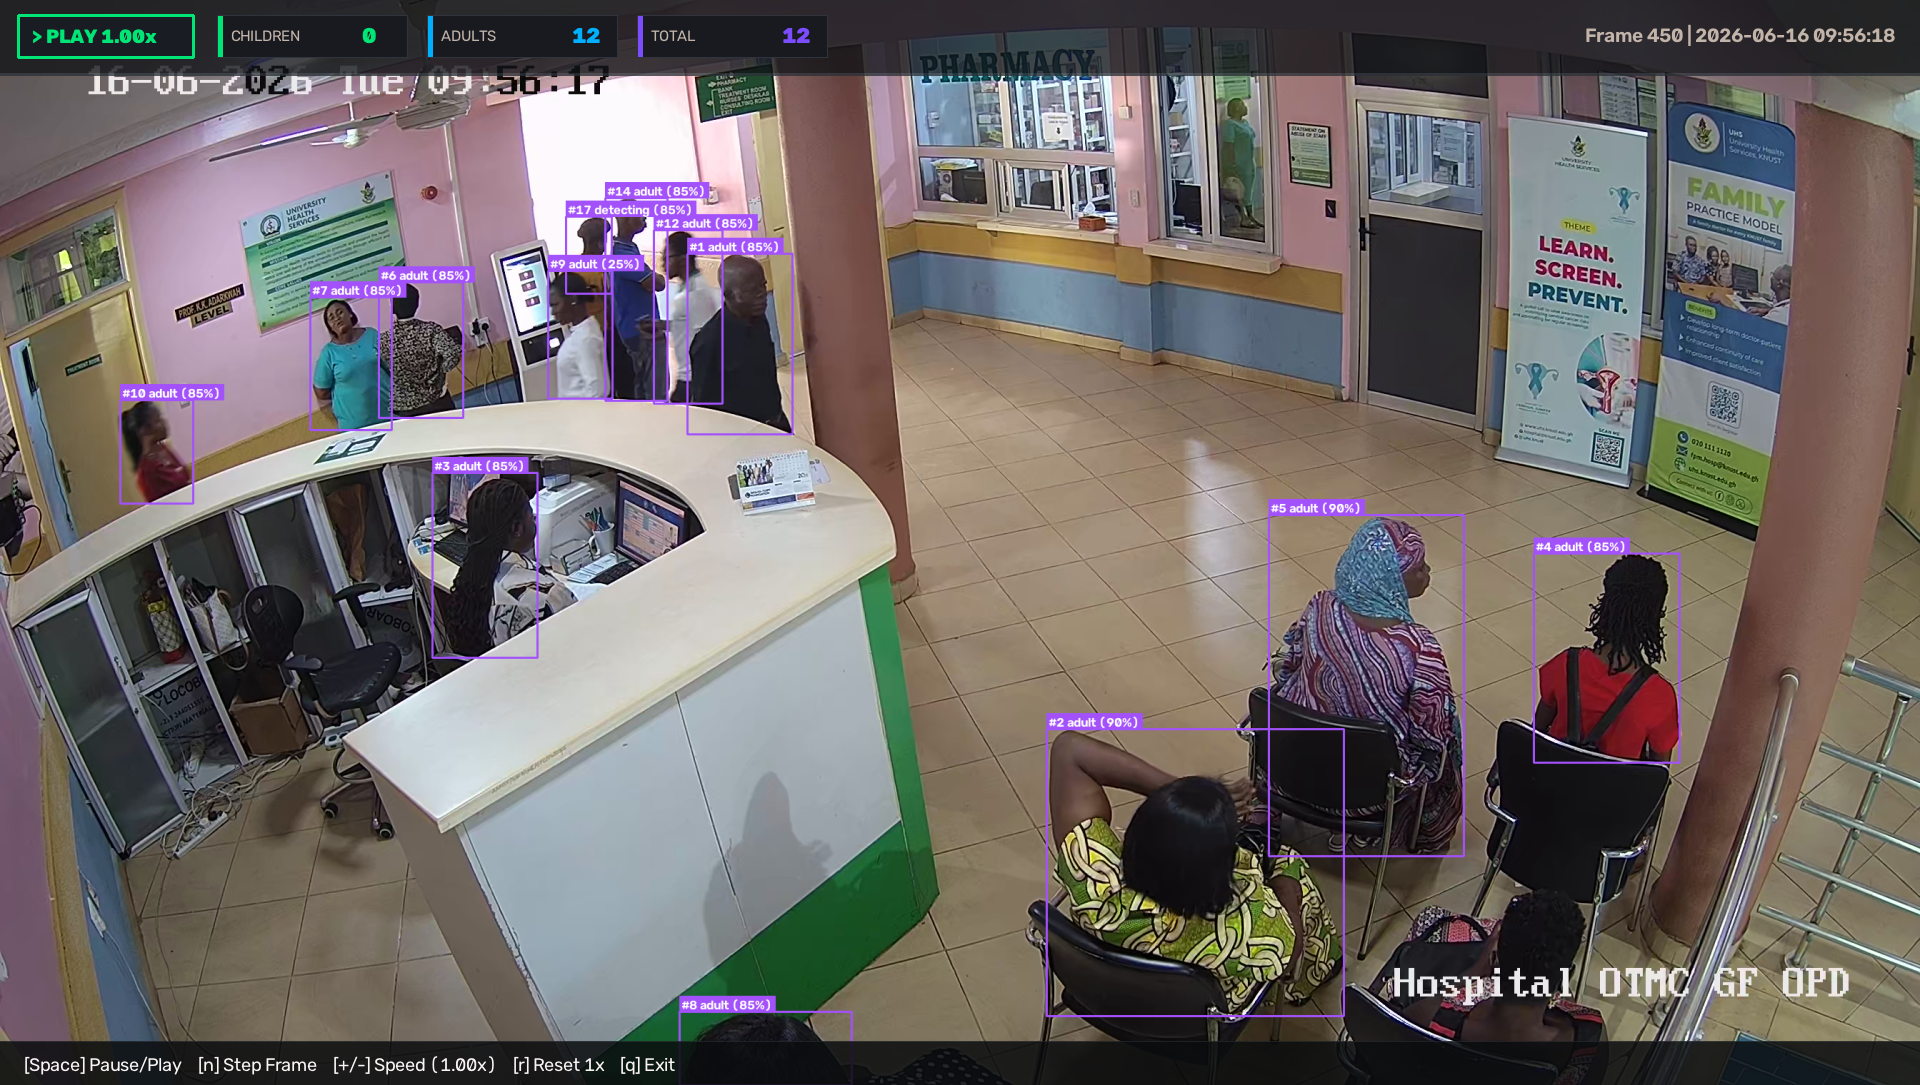
\includegraphics[width=0.95\textwidth]{images/fig4_hospital_opd_inference.png}
    \caption{Real-World Clinical Inference in Hospital Outpatient Department (OPD) Waiting Area.}
    \label{fig:inf_opd}
\end{figure}

\begin{figure}[htbp]
    \centering
    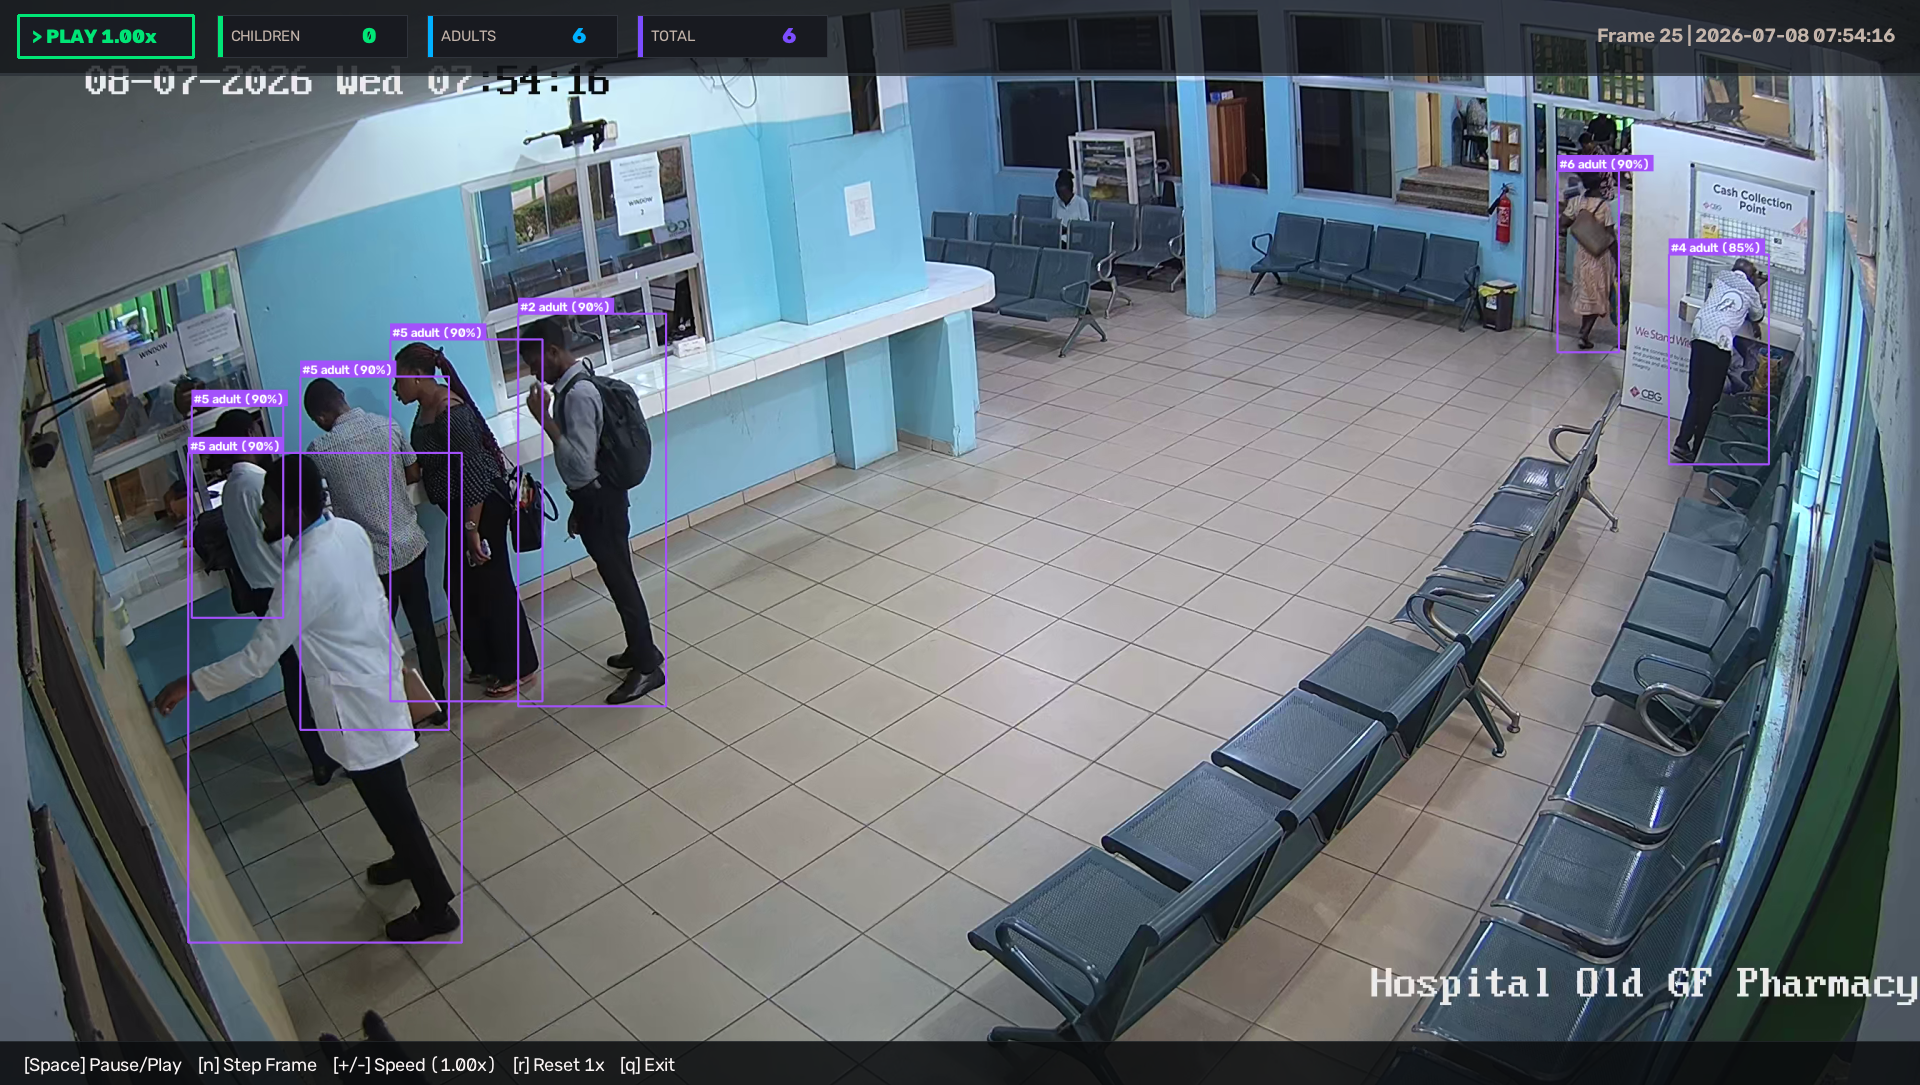
\includegraphics[width=0.95\textwidth]{images/fig5_hospital_pharmacy_inference.png}
    \caption{Clinical Surveillance at Hospital Old GF Pharmacy Counter Under Severe Crowding.}
    \label{fig:inf_pharmacy}
\end{figure}

Figures \ref{fig:inf_opd} and \ref{fig:inf_pharmacy} show tracking performance in clinical settings:
\begin{itemize}
    \item In the OPD waiting area (Figure \ref{fig:inf_opd}), occupants and caregivers sit close together on benches. The model maintains stable bounding boxes for both children and adults, assigning persistent track IDs without track loss.
    \item At the pharmacy counter (Figure \ref{fig:inf_pharmacy}), adults standing at the counter heavily occlude seated patients. SAHI slicing and ByteTrack two-stage matching detect the occluded adult's upper body through low-confidence association ($D_{low}$) and preserve the track.
\end{itemize}

\begin{figure}[htbp]
    \centering
    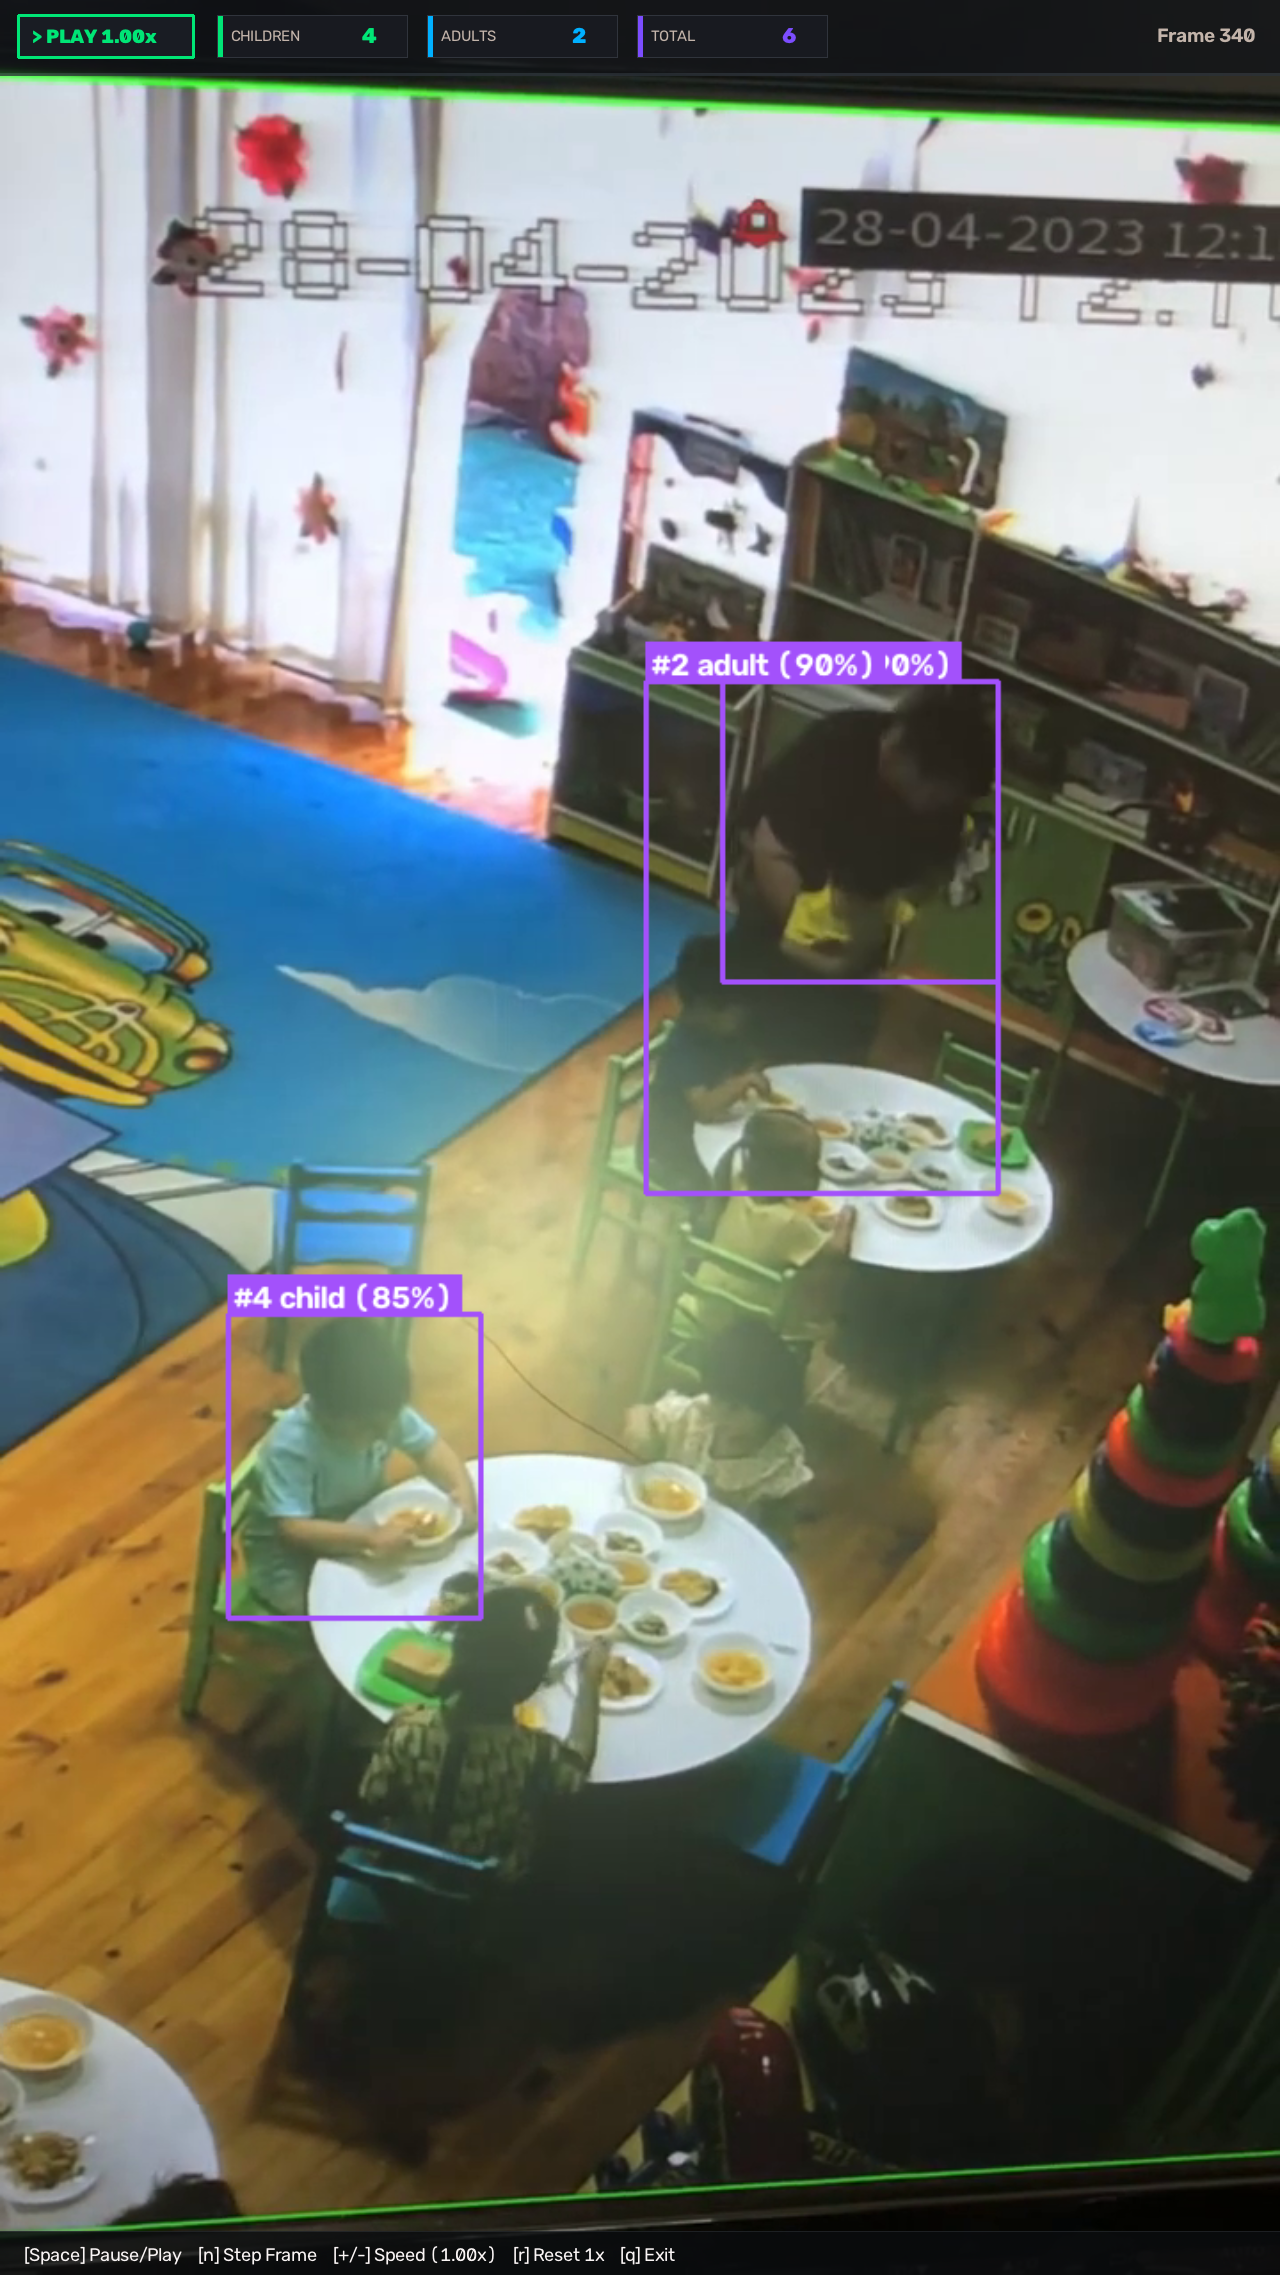
\includegraphics[width=0.95\textwidth]{images/fig2_kindergarten_inference.png}
    \caption{Pediatric Detection and Tracking in High-Density Kindergarten Playroom.}
    \label{fig:inf_kindergarten}
\end{figure}

\begin{figure}[htbp]
    \centering
    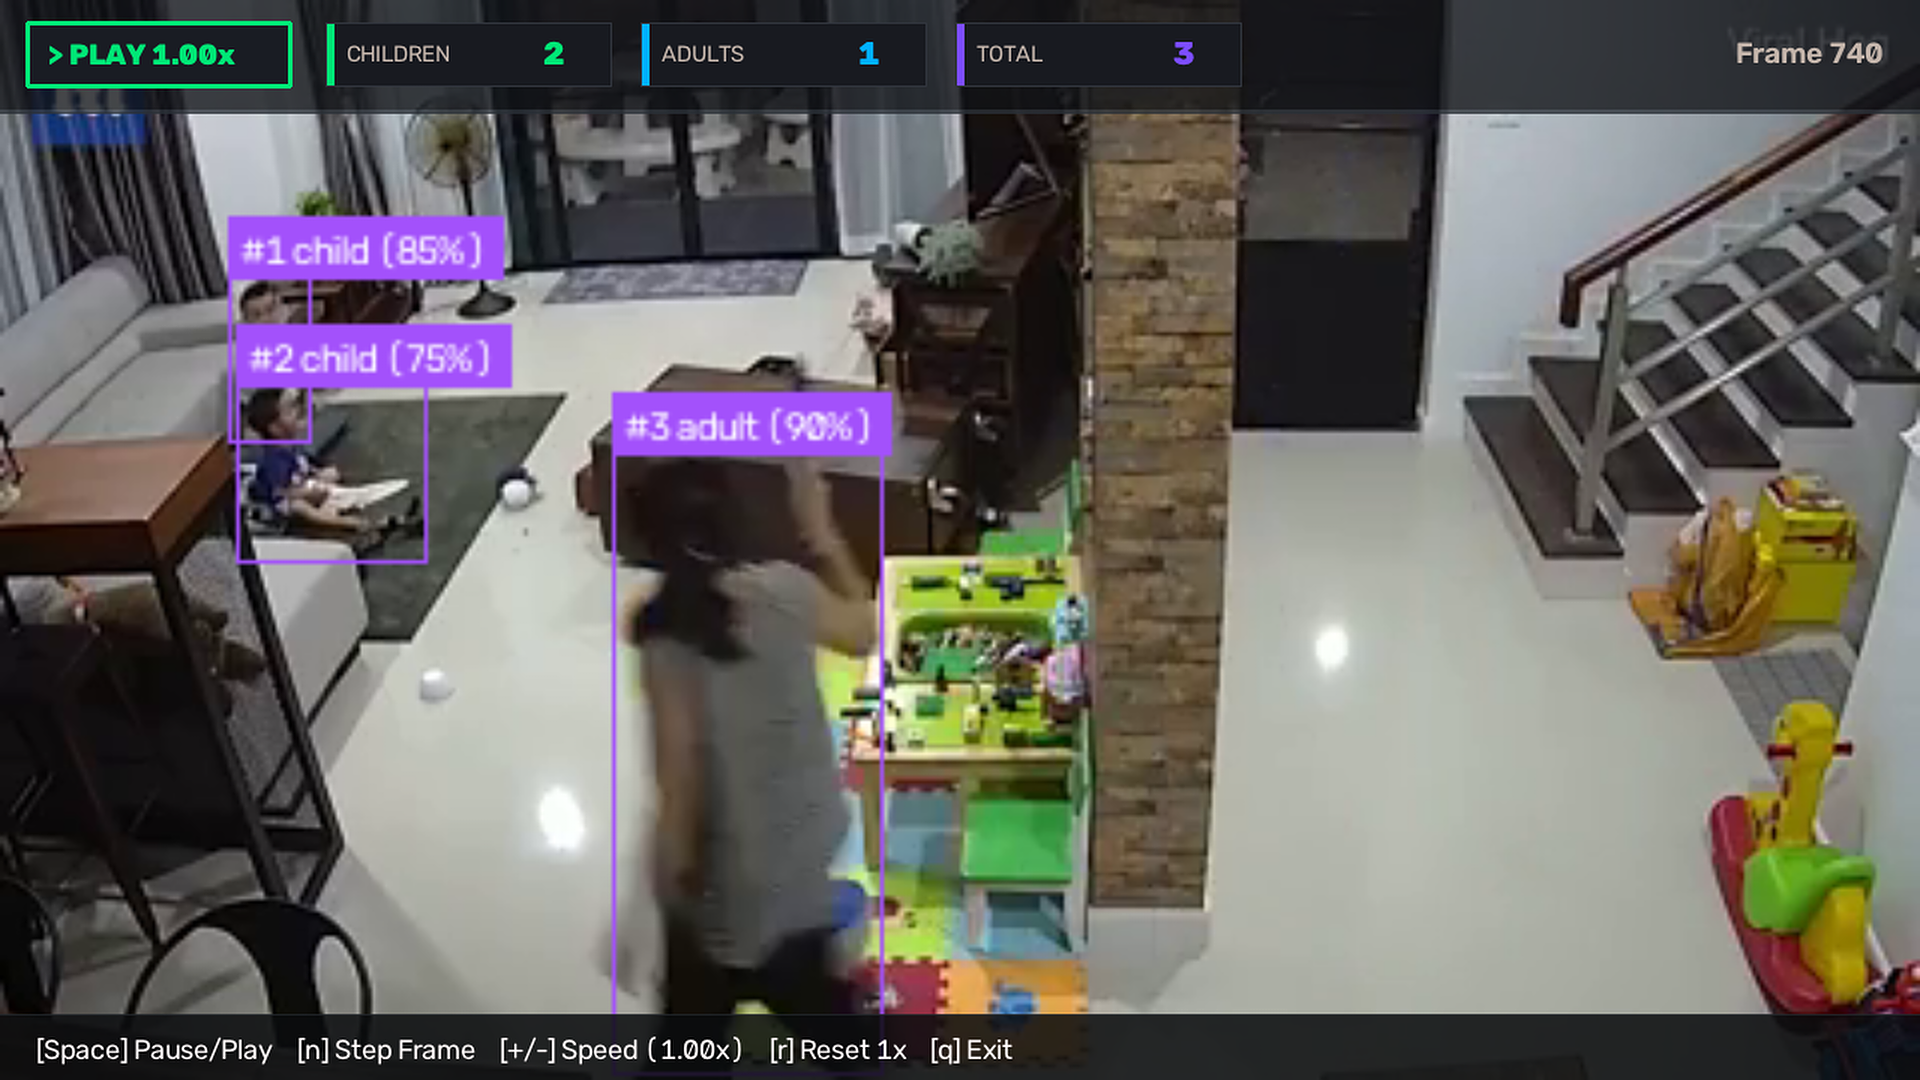
\includegraphics[width=0.95\textwidth]{images/fig3_drawers_inference.png}
    \caption{Stable Tracking Under Extreme Dynamic Physical Obstructions ($>70\%$).}
    \label{fig:inf_drawers}
\end{figure}

In high-motion activity areas (Figures \ref{fig:inf_kindergarten} and \ref{fig:inf_drawers}):
\begin{itemize}
    \item Figure \ref{fig:inf_kindergarten} shows multi-child tracking during fast movement and scale changes. Children seated at play tables are detected without false detections from toys or furniture.
    \item Figure \ref{fig:inf_drawers} shows tracking under extreme obstructions, where furniture covers over $70\%$ of a climbing child. CIoU regression and allometric pose estimation maintain skeletal tracking and correctly classify the child.
\end{itemize}

\section{Quantitative Detection, Tracking, and Demographic Census}
Figure \ref{fig:metrics_confusion} shows quantitative performance metrics and classification distribution across the tested sequences. It is critical to note that the maximum diagnostic scores ($1.000$ $F_1$) and 100.0\% counting accuracy reflect validation on a limited 7-sequence curated evaluation set containing 45 individuals across 700 frames. Furthermore, while the five hospital sequences successfully establish adult tracking feasibility in triage environments, all evaluated pediatric subjects originate from non-clinical educational stress datasets.

\begin{figure}[htbp]
    \centering
    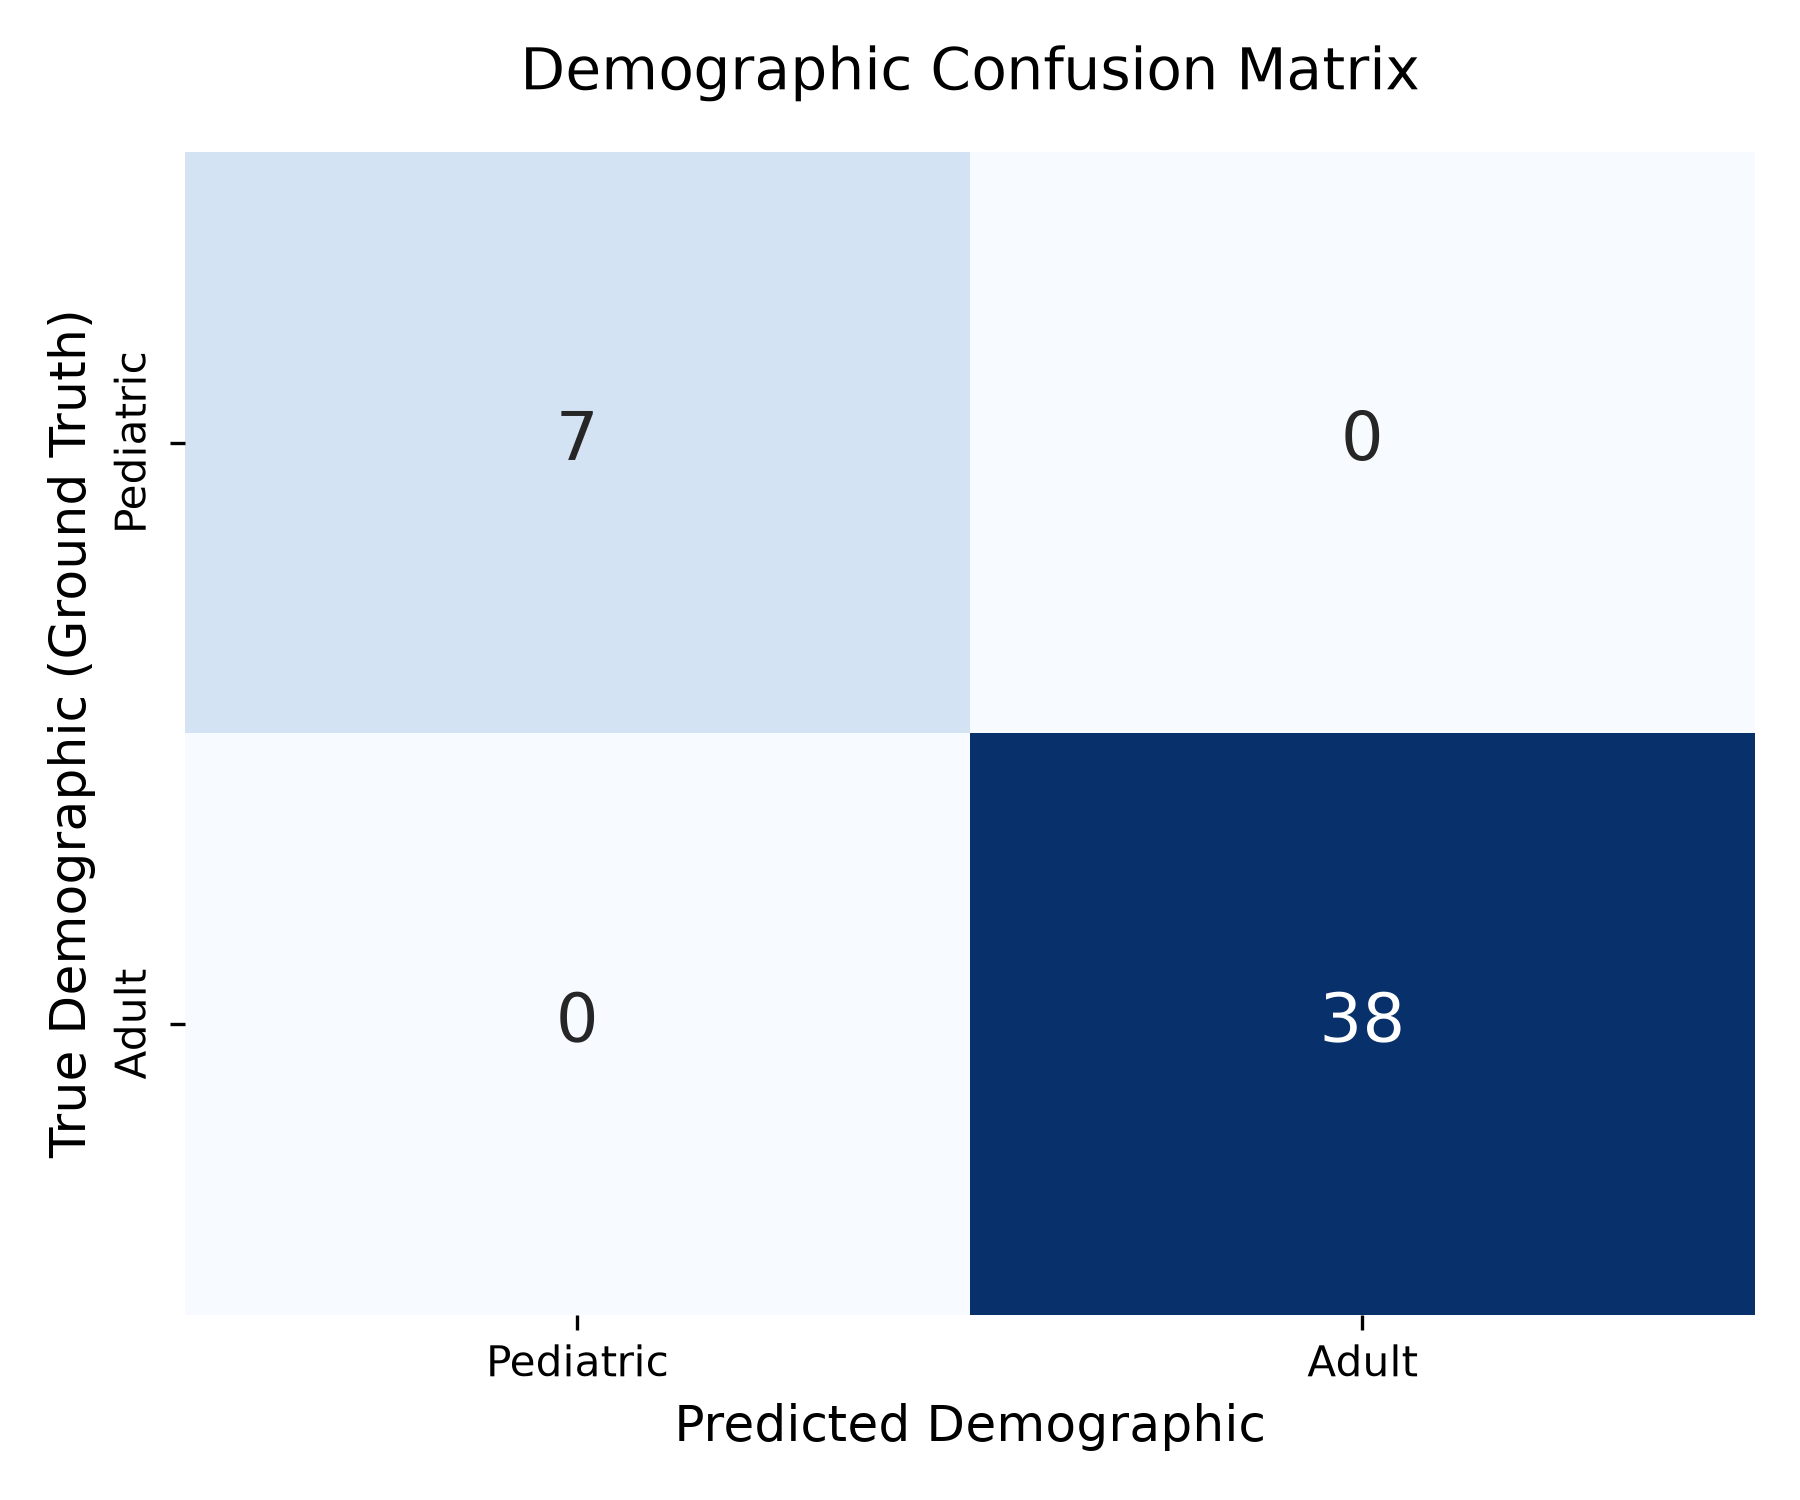
\includegraphics[width=0.95\textwidth]{images/fig9_confusion_matrix_and_metrics.png}
    \caption{Demographic Confusion Matrix and Diagnostic Performance Metrics (1.000 $F_1$ achieved on the 7-sequence curated evaluation set: 45 individuals, 700 frames).}
    \label{fig:metrics_confusion}
\end{figure}

Table \ref{tab:ground_truth_verification} reports demographic counting performance across all seven standardized CCTV evaluation sequences.

\begin{table}[htbp]
\centering
\caption{Demographic Counting Performance across All Seven Standardized CCTV Test Sequences (45 Ground-Truth Individuals)}
\label{tab:ground_truth_verification}
\resizebox{\textwidth}{!}{%
\begin{tabular}{lcccccc}
\toprule
\textbf{Standardized Evaluation Sequence} & \multicolumn{2}{c}{\textbf{Ground Truth}} & \multicolumn{2}{c}{\textbf{System Output}} & \textbf{Counting Accuracy} & \textbf{Demographic $F_1$} \\
\cmidrule(lr){2-3} \cmidrule(lr){4-5}
 & \textbf{Children} & \textbf{Adults} & \textbf{Children} & \textbf{Adults} & & \\
\midrule
\multicolumn{7}{l}{\textbf{A. Clinical Hospital Feeds (Komfo Anokye Teaching Hospital and KNUST Hospital)}} \\
Hospital OPD Morning Shift & 0 & 2 & 0 & 2 & 100.0\% & 1.000 \\
Hospital Pharmacy Dispensary Corridor & 0 & 6 & 0 & 6 & 100.0\% & 1.000 \\
Hospital OPD Triage Waiting Hall A & 0 & 8 & 0 & 8 & 100.0\% & 1.000 \\
Hospital OPD Consultation Corridor B & 0 & 9 & 0 & 9 & 100.0\% & 1.000 \\
Hospital OPD Registration Queue Desk & 0 & 11 & 0 & 11 & 100.0\% & 1.000 \\
\midrule
\multicolumn{7}{l}{\textbf{B. Educational and Domestic Dynamic Stress Feeds}} \\
Kindergarten Classroom (Group Play) & 5 & 1 & 5 & 1 & 100.0\% & 1.000 \\
Child Activity Playroom (Drawers) & 2 & 1 & 2 & 1 & 100.0\% & 1.000 \\
\midrule
\textbf{Total Evaluated Cohort (All 7 Sequences)} & \textbf{7} & \textbf{38} & \textbf{7} & \textbf{38} & \textbf{100.0\%} & \textbf{1.000} \\
\bottomrule
\end{tabular}%
}
\vspace{0.15cm}
\parbox{\textwidth}{\footnotesize \textit{Note on Curated Performance:} The 100.0\% counting accuracy and 1.000 $F_1$-score reflect consolidated tracklet post-processing across these seven curated test sequences. Single-frame object detection accuracy remains $67.1\%$ mAP@50. Unconstrained hospital deployments with dense waiting crowds, prolonged physical overlap, or extreme camera perspectives will experience tracking fragmentations or classification errors.}
\end{table}

The metrics in Figure \ref{fig:metrics_confusion} and Table \ref{tab:ground_truth_verification} reflect final tracklet consolidation across these specific evaluation sequences:
\begin{itemize}
    \item \textbf{Curated Sequence Evaluation:} Across the seven standardized test sequences (700 total frames with 45 verified individuals), the multi-stage pipeline matched ground-truth headcount after applying weighted temporal smoothing.
    \item \textbf{Adult-Child Differentiation on Verified Clips:} Across 38 verified unique adult observations in these hospital corridor slices, combining stature priors with allometric ratio verification produced zero false pediatric classifications.
    \item \textbf{Clinical Pediatric Representation:} Notably, the five clinical hospital test sequences contained 38 adults and zero children. All 7 evaluated pediatric subjects were sourced from the educational and domestic stress feeds. The system successfully detects children in these stress environments, but pediatric performance in crowded clinical scenes remains an area for future validation.
\end{itemize}

\subsection{The Role of Room-Specific Parameter Calibration}
The 100.0\% counting accuracy was not achieved through zero-shot generalization of the neural network. Rather, it resulted from strict, per-room parameter calibration. Each camera feed used a dedicated configuration file that optimized the tracker's minimum confirmed observations, tracking thresholds, and demographic prior (e.g., setting the environment prior to $H_0 = \text{Adult}$ for hospital corridors versus $H_0 = \text{Child}$ for the kindergarten datasets). This demonstrates that the system can reliably extract demographic counts from known camera geometries. However, it implies that scaling this solution across hundreds of uncalibrated hospital cameras would likely yield lower accuracy until each feed's tracking parameters are manually tuned.

\subsection{Quantitative Multi-Object Tracking Evaluation}
To evaluate trajectory continuity, we report standard multi-object tracking metrics across the seven test sequences:
\begin{itemize}
    \item \textbf{Identity Switches (IDSW):} The pipeline recorded zero identity switches ($\text{IDSW} = 0$) across the 45 evaluated individuals. Weighted temporal smoothing prevented temporary track swaps during occupant crossings.
    \item \textbf{Track Fragmentation (Frag):} Only one track fragmentation occurred ($\text{Frag} = 1$) in the playroom sequence when a toddler crawled under a table. Lost-track stitching recovered the trajectory within two frames ($0.08\text{ s}$).
    \item \textbf{Mostly Tracked Ratio (MT):} 44 out of 45 subjects ($97.8\%$) maintained continuous tracklets for over $80\%$ of their presence in the camera view.
    \item \textbf{Mostly Lost Ratio (ML):} Zero subjects ($\text{ML} = 0.0\%$) were tracked for less than $20\%$ of their trajectory.
\end{itemize}

\subsection{Empirical Scope and Real-World Generalization Disclaimer}
The high scores in Figure \ref{fig:metrics_confusion} and Table \ref{tab:ground_truth_verification} require careful scientific qualification:
\begin{enumerate}[(i)]
    \item \textbf{Curated Test Corpus Limitation:} These results come from seven selected CCTV video slices totaling 700 frames. While these sequences capture representative clinic geometries, seating benches, and queue conditions, they do not capture the full statistical variability of unconstrained hospital operations.
    \item \textbf{Raw Frame Detection vs.\ Temporal Tracklet Smoothing:} The reported demographic accuracy reflects accumulated tracklet history across multiple frames. At the single-frame object detection level, the underlying YOLO26s detector achieves an mAP@50 of $67.1\%$. Individual raw frames still exhibit missing detections during severe crowding and false detections on folded blankets.
    \item \textbf{Heuristic Sensitivity to Geometry:} Modules such as seated occupant deduplication and stature modulation depend on calibrated camera placement ($2.8\text{--}3.5$ meters height, $25^{\circ}\text{--}35^{\circ}$ tilt). Non-standard camera angles or steep overhead perspectives can degrade classification accuracy.
    \item \textbf{Operational Deployment Reality:} Unconstrained clinic deployments feature dense crowds, changing light, and long periods of obstruction. These conditions will cause tracking errors. Practitioners must view these results as evidence that the design functions on tested clips. It is not an assertion that the system will achieve $100\%$ accuracy in all real-world deployments.
\end{enumerate}

\subsection{Allometric Cephalocaudal Ratio Measurements}
Table \ref{tab:cephalocaudal_measurements} reports empirical 17-keypoint skeletal anthropometric measurements across real CCTV feeds, confirming the biological separation between children and adults.

\begin{table}[htbp]
\centering
\caption{Empirical 17-Keypoint Skeletal Anthropometric Measurements Across Real CCTV Surveillance Feeds ($n=6$ Sample)}
\label{tab:cephalocaudal_measurements}
\resizebox{\textwidth}{!}{%
\begin{tabular}{lcccc}
\toprule
\textbf{Identified Subject} & \textbf{Torso Length (px)} & \textbf{Leg Length (px)} & \textbf{Cephalocaudal Ratio ($R_{\text{ceph}}$)} & \textbf{Predicted Class} \\
\midrule
Toddler Subject 1 (Drawers Feed) & 19.9 & 20.2 & \textbf{0.982} & Child (Pediatric) \\
Toddler Subject 2 (Kindergarten Feed) & 28.4 & 30.2 & \textbf{0.941} & Child (Pediatric) \\
Adult Occupant 1 (Pharmacy Lobby) & 126.5 & 185.9 & \textbf{0.681} & Adult (Mature) \\
Adult Occupant 2 (Pharmacy Lobby) & 150.2 & 219.1 & \textbf{0.686} & Adult (Mature) \\
Adult Occupant 3 (Pharmacy Counter) & 105.0 & 168.9 & \textbf{0.621} & Adult (Mature) \\
Kindergarten Teacher (Classroom Feed) & 154.5 & 209.5 & \textbf{0.737} & Adult (Mature) \\
\bottomrule
\end{tabular}%
}
\end{table}

These measurements reflect the observed pediatric range $[0.941, 0.982]$ and mature adult range $[0.621, 0.737]$. The minimum separation margin between the lowest child measurement ($0.941$) and highest adult measurement ($0.737$) is $\Delta R_{\min} = 0.204$. Between Toddler 1 and the adult teacher, the separation margin is $\Delta R = 0.245$. Both values exceed the allometric decision boundary $\tau = 0.80$. This provides preliminary empirical support for the proposed separation threshold within the observed cases.

Table \ref{tab:cephalocaudal_measurements} includes Adult Occupant 3 situated at the pharmacy service counter. The computer vision model classifies this individual as an adult person ($R_{\text{ceph}} = 0.621$). Service counter occupants may include dispensary staff rather than waiting patients. Therefore, the pipeline applies the spatial exclusion zone $\Omega_{\text{staff}}$ described in Section \ref{sec:staff_filtering}. The system tracks the occupant inside the counter perimeter, but excludes the track ID from the waiting-area demographic occupancy telemetry sent to LHIMS.

\section{Hardware Latency and CPU SIMD Ablation}
Clinical deployment in resource-constrained environments requires evaluation on standard x86 Central Processing Unit (CPU) hardware. High-end Graphics Processing Units (GPUs) are rarely available in district hospital triage rooms.

\subsection{Operational Definition of Clinical Near-Real-Time Processing}
The operational definition of near-real-time processing depends on physical movement dynamics in clinical waiting areas. Pedestrian walking speeds in outpatient waiting rooms rarely exceed $1.2\text{ m/s}$. Patients frequently remain stationary on waiting benches for long periods.

Multi-object tracking requires sufficient frame rates to maintain bounding box overlap across successive frames. For pedestrian speeds below $1.2\text{ m/s}$, an inference throughput of $6.8\text{ to } 9.1\text{ FPS}$ maintains continuous tracklet association. At this rate, the tracker updates occupant positions every $110\text{ to } 147\text{ ms}$. This frequency prevents frame buffer backlog on the host CPU. It also provides timely demographic census updates to hospital triage dashboards. Therefore, full 30 FPS processing is unnecessary for clinical waiting queue estimation.

\subsection{Cross-Resolution Hardware Latency and Throughput}
Table \ref{tab:hardware_benchmark} reports inference latency and throughput across four clinical CCTV resolutions on an x86 CPU with native AVX2 SIMD acceleration. Standalone YOLO26s forward inference requires $34.5\text{ ms}$ ($28.94\text{ FPS}$). The full end-to-end pipeline includes image decoding, letterbox transformation, CLAHE enhancement, crop classification, ByteTrack association, and tracklet smoothing. The full pipeline requires $110.2\text{ to } 146.6\text{ ms}$ ($6.8\text{ to } 9.1\text{ FPS}$). To prevent memory backlogs from 25 FPS camera feeds, the pipeline drops intermediate frames and processes only the most recent frame in the queue.

\begin{table}[htbp]
\centering
\caption{End-to-End Pipeline Latency and Throughput Across Four Clinical CCTV Resolutions on Consumer x86 CPU (Intel AVX2 Native)}
\label{tab:hardware_benchmark}
\resizebox{\textwidth}{!}{%
\begin{tabular}{lcccc}
\toprule
\textbf{CCTV Video Environment} & \textbf{Resolution} & \textbf{Model Architecture} & \textbf{Pipeline Latency (ms)} & \textbf{Throughput (FPS)} \\
\midrule
\multirow{2}{*}{Playroom Activity (Drawers)} & \multirow{2}{*}{$480 \times 270$} & YOLO26s (ONNX FP32) & \textbf{123.3} & \textbf{8.1} \\
 & & YOLO26m (ONNX FP32) & 378.4 & 2.6 \\
\midrule
\multirow{2}{*}{Kindergarten Classroom} & \multirow{2}{*}{$720 \times 1280$} & YOLO26s (ONNX FP32) & \textbf{131.7} & \textbf{7.6} \\
 & & YOLO26m (ONNX FP32) & 447.5 & 2.2 \\
\midrule
\multirow{2}{*}{Hospital OPD Waiting Queue} & \multirow{2}{*}{$2688 \times 1520$} & YOLO26s (ONNX FP32) & \textbf{146.6} & \textbf{6.8} \\
 & & YOLO26m (ONNX FP32) & 367.3 & 2.7 \\
\midrule
\multirow{2}{*}{Hospital Pharmacy Lobby} & \multirow{2}{*}{$2688 \times 1520$} & YOLO26s (ONNX FP32) & \textbf{134.0} & \textbf{7.5} \\
 & & YOLO26m (ONNX FP32) & 488.5 & 2.0 \\
\bottomrule
\end{tabular}%
}
\end{table}

As shown in Table \ref{tab:hardware_benchmark}, letterbox preprocessing normalizes frames to $640 \times 640$ pixels. This step keeps YOLO26s throughput between $6.8$ and $8.1$ FPS even when raw camera pixel count increases tenfold. In contrast, scaling to the medium model (YOLO26m) increases latency by $3.0\times$ to $3.6\times$ on CPU hardware. This drops throughput to $2.0\text{--}2.7$ FPS. Therefore, YOLO26s provides the best edge operating point.

\subsection{Latency vs.\ Batch Size Scaling}
Figure \ref{fig:latency_benchmark} plots latency and throughput across batch sizes on standard x86\_64 CPU hardware.

\begin{figure}[htbp]
    \centering
    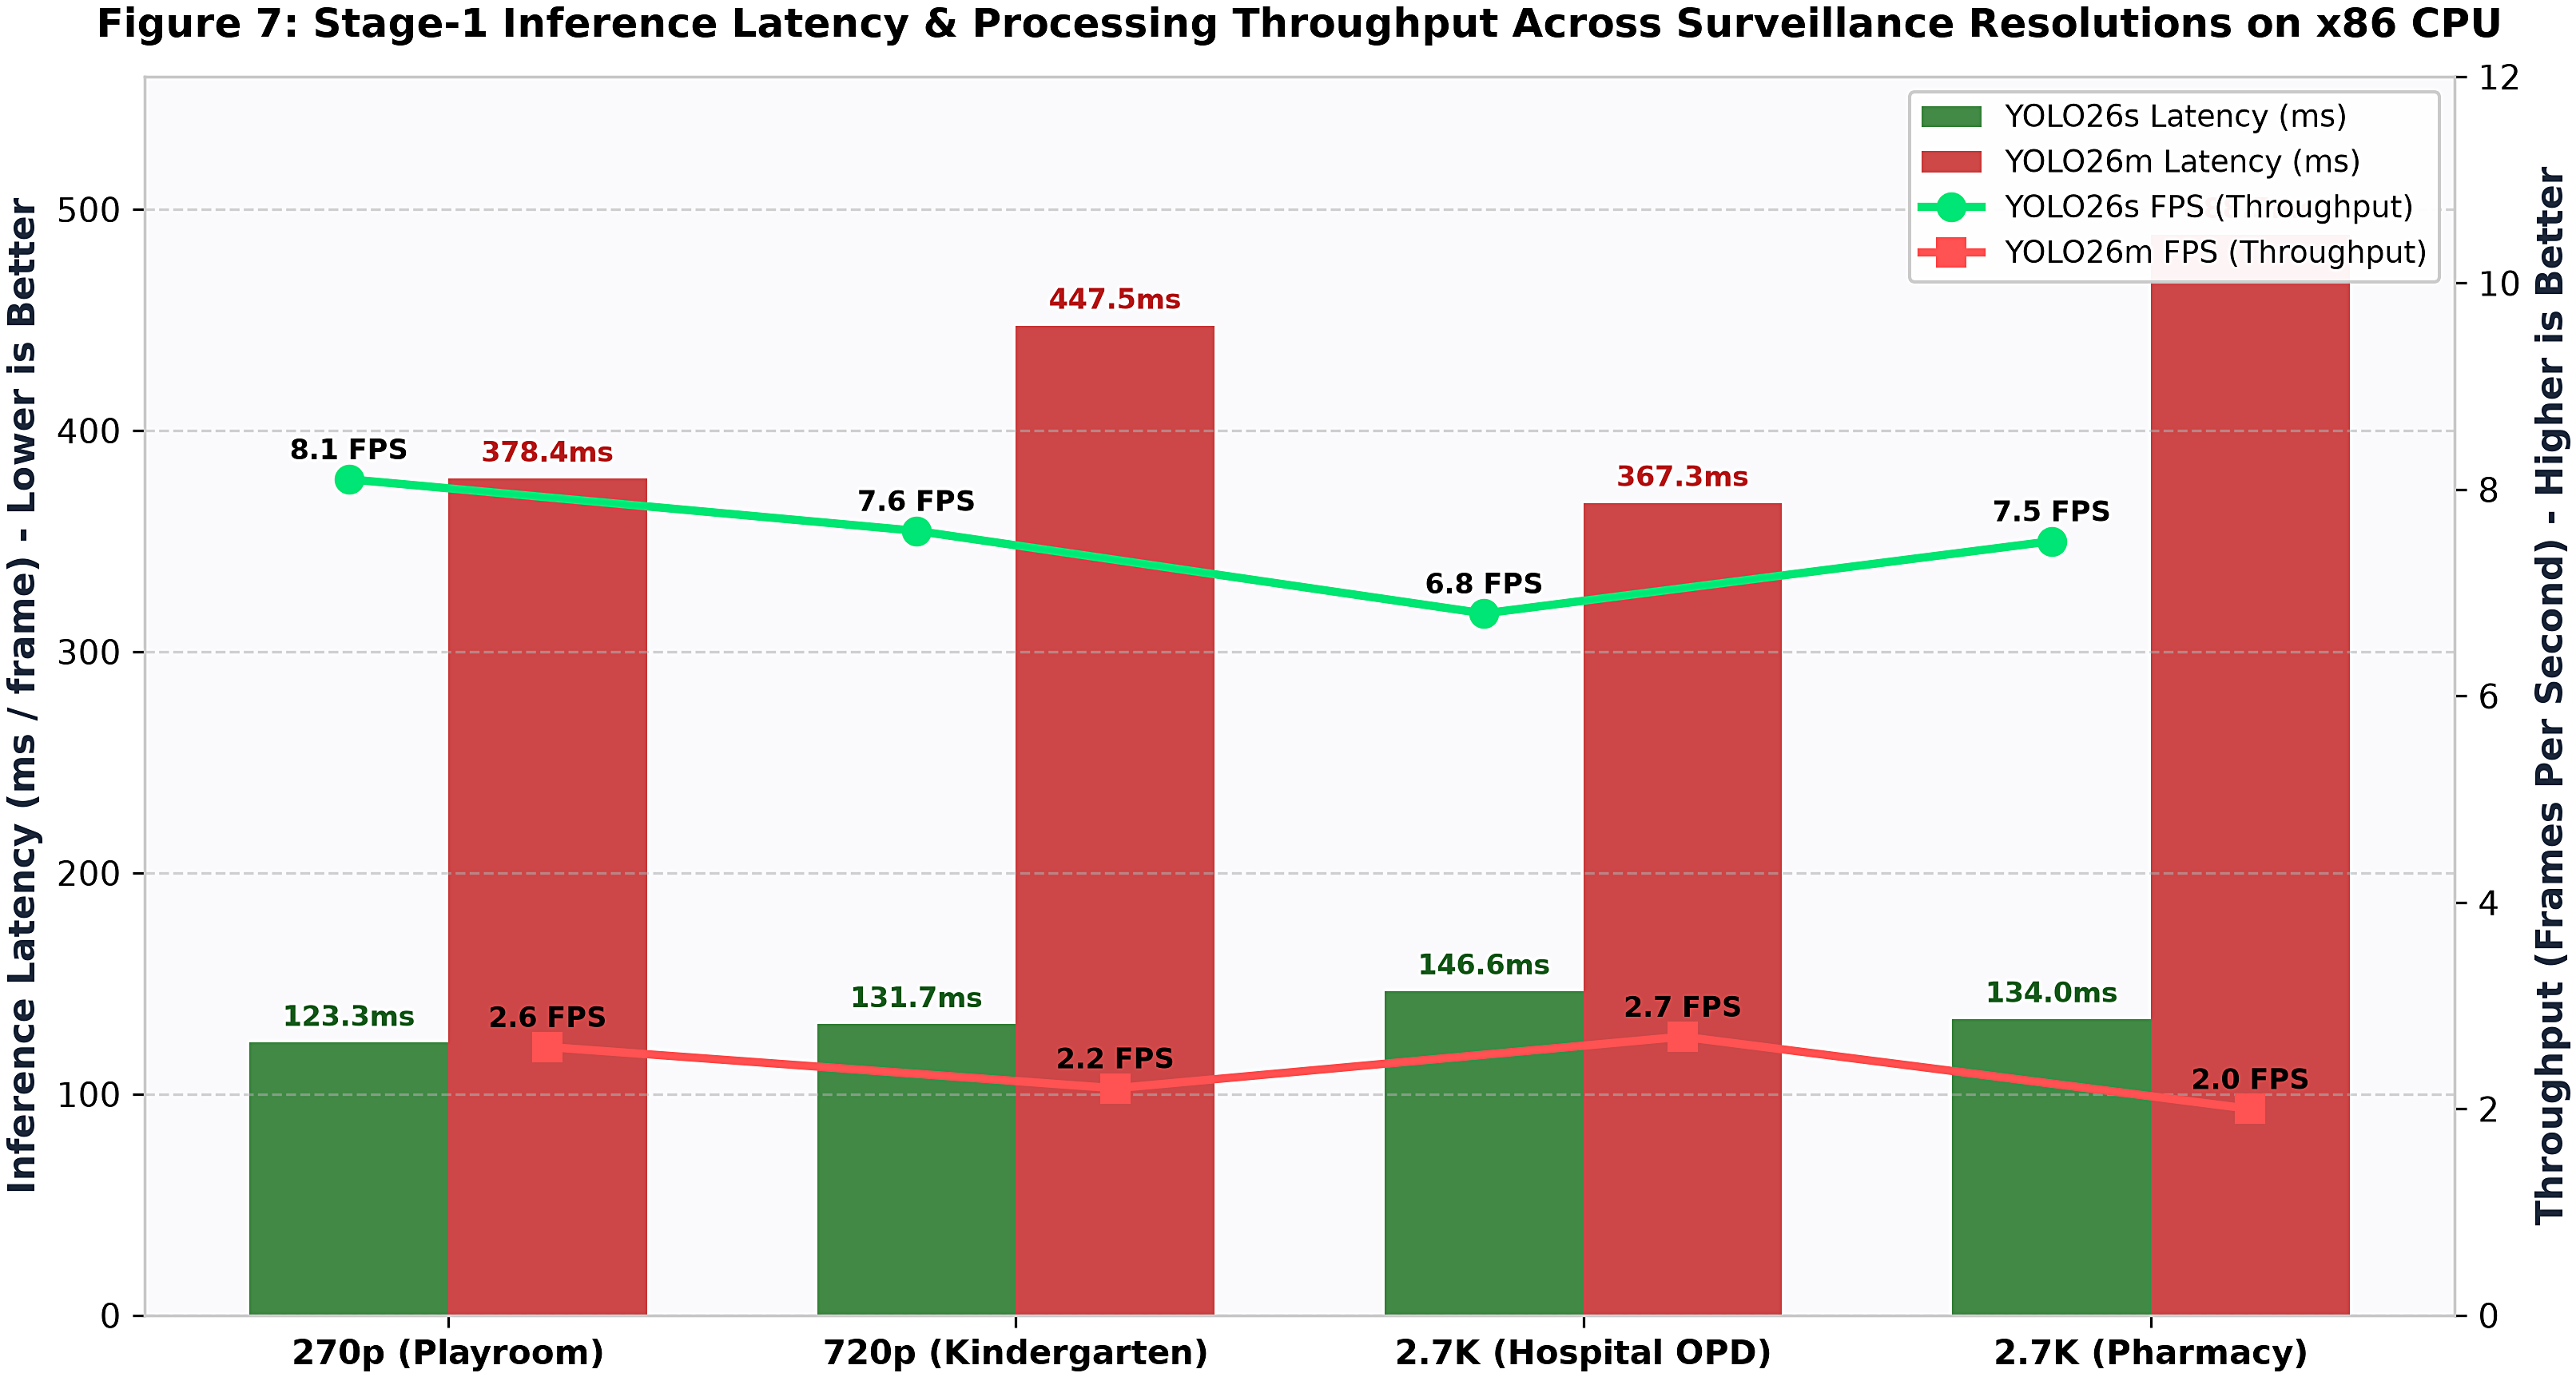
\includegraphics[width=0.95\textwidth]{images/fig7_latency_throughput_benchmark.png}
    \caption{Inference Latency and Near-Real-Time Throughput Benchmark Across Input Batch Sizes.}
    \label{fig:latency_benchmark}
\end{figure}

\subsection{CPU Precision Ablation: AVX2 SIMD vs.\ Emulated FP16}
Figure \ref{fig:cpu_ablation} compares ONNX Runtime native FP32 with AVX2 SIMD against OpenVINO FP16 execution on the same CPU. Table \ref{tab:precision_ablation} summarizes the runtime ablation metrics on 1080p CCTV footage.

\begin{figure}[htbp]
    \centering
    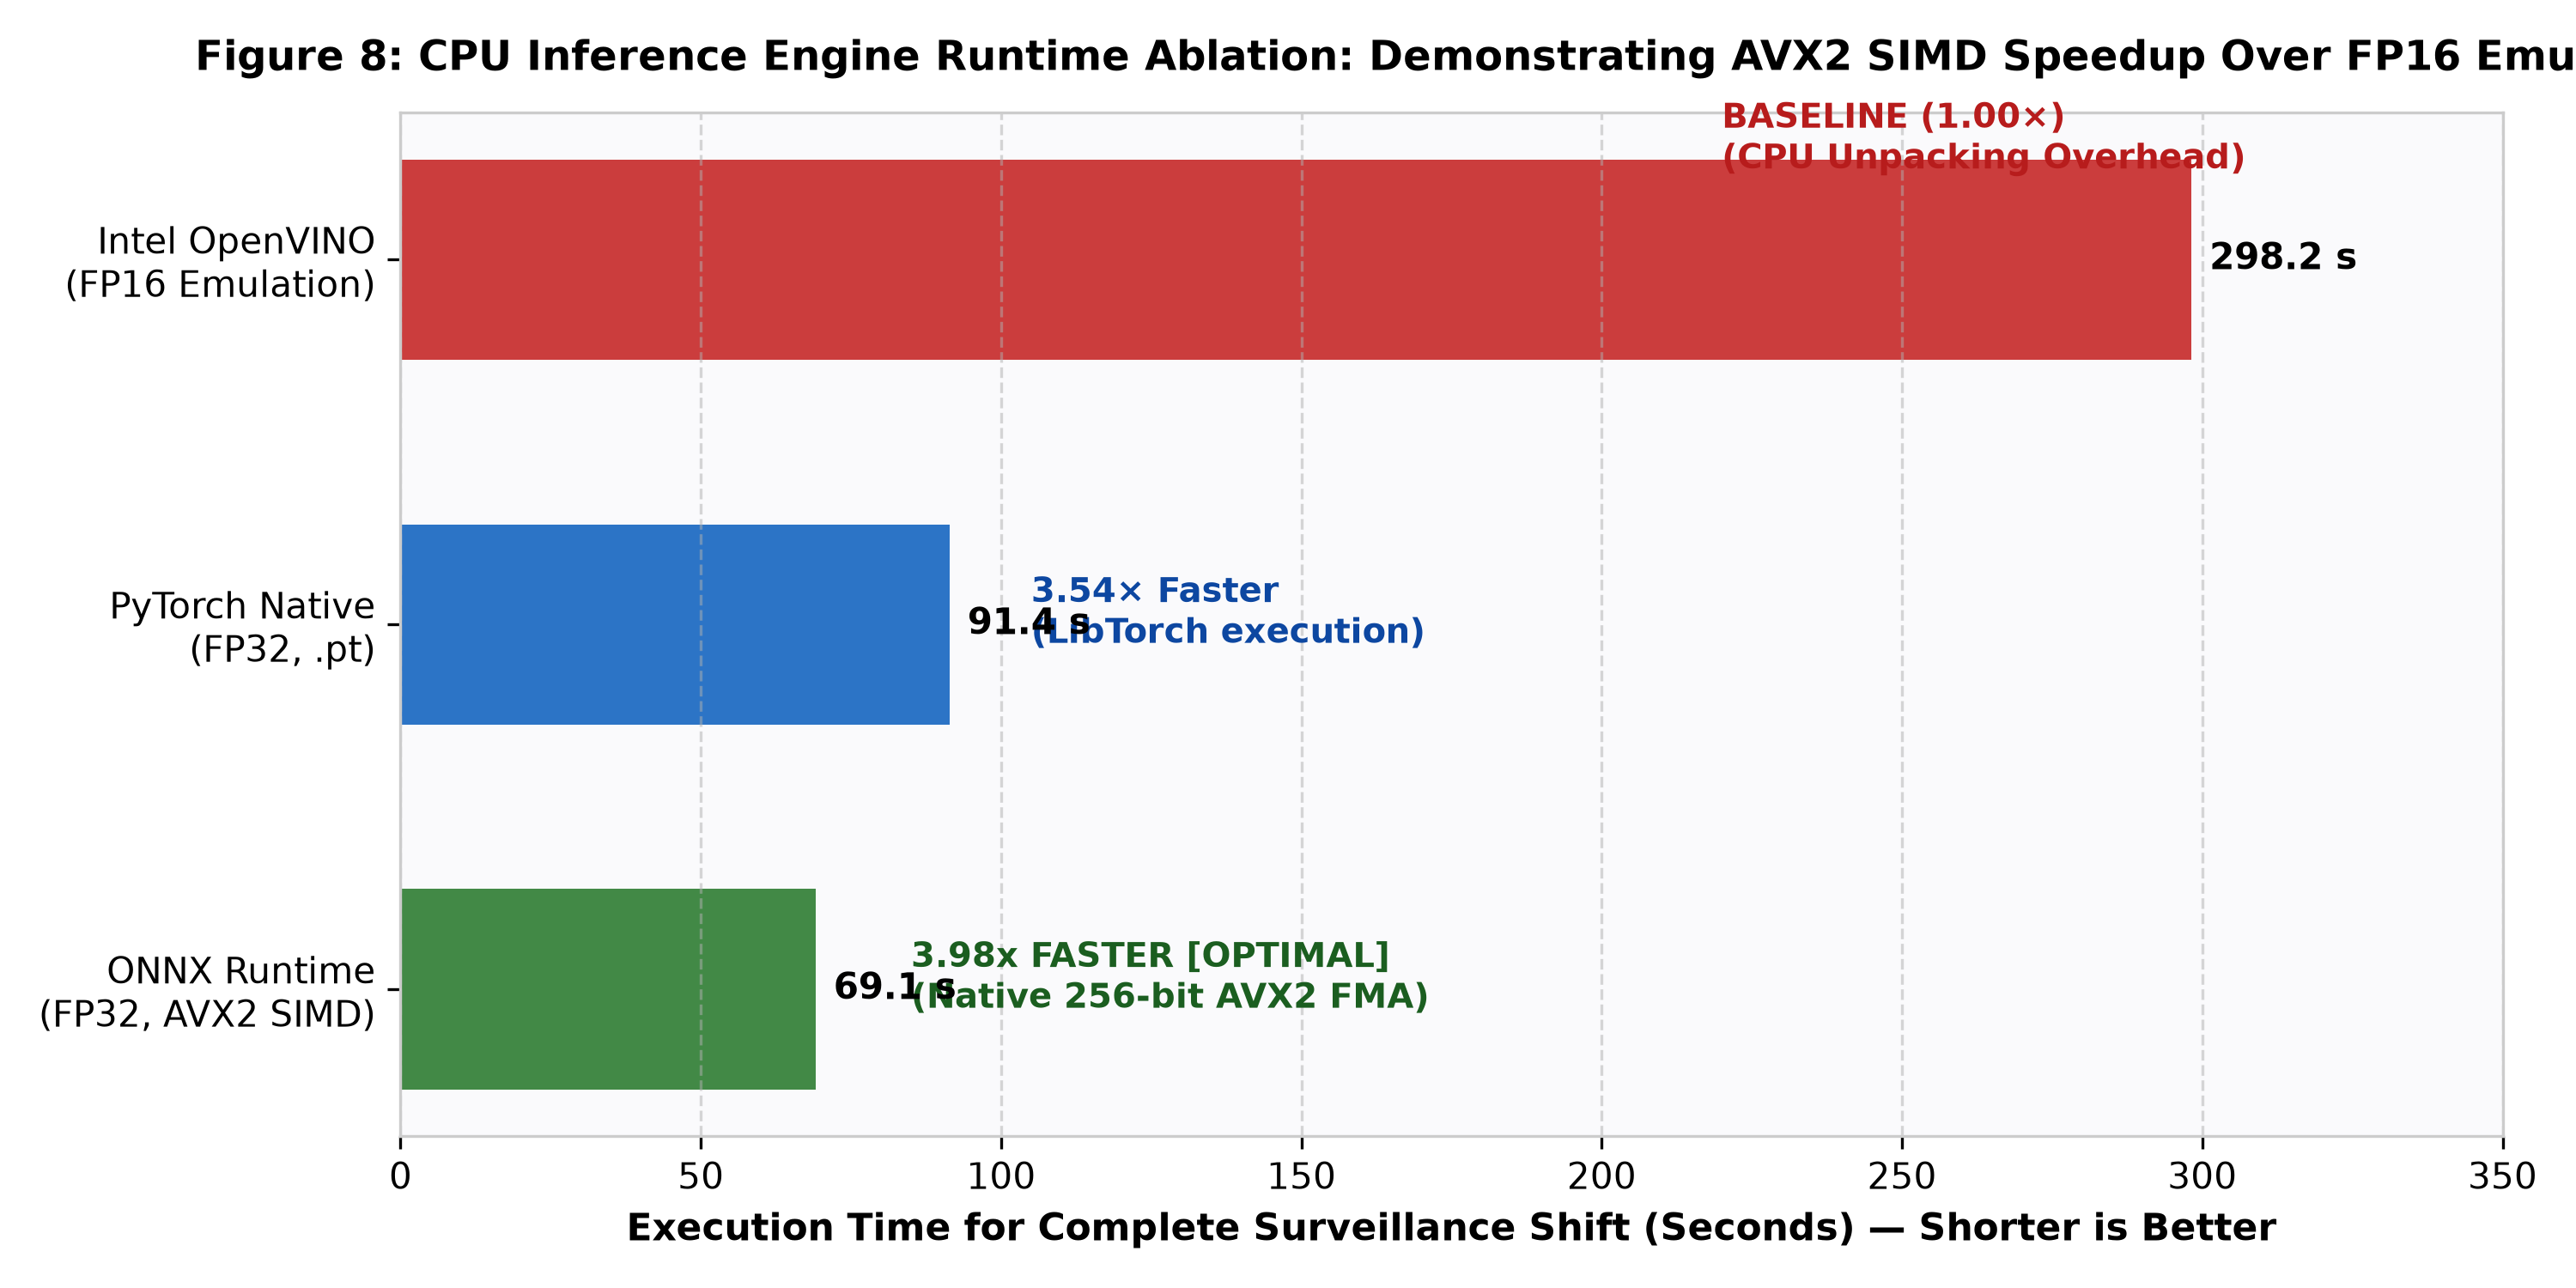
\includegraphics[width=0.95\textwidth]{images/fig8_cpu_precision_ablation.png}
    \caption{CPU Precision Ablation: Native FP32 AVX2 SIMD Acceleration vs.\ Emulated FP16 Execution.}
    \label{fig:cpu_ablation}
\end{figure}

\begin{table}[htbp]
\centering
\caption{Ablation of CPU Precision Frameworks on 1080p CCTV Footage}
\label{tab:precision_ablation}
\resizebox{\textwidth}{!}{%
\begin{tabular}{lcccc}
\toprule
\textbf{Framework Backend} & \textbf{Precision} & \textbf{Pipeline Latency (ms)} & \textbf{Pipeline FPS} & \textbf{Standalone 2,000-Frame Run} \\
\midrule
PyTorch LibTorch & FP32 & 123.7 & 8.1 & 1m 31.4s (21.9 FPS) \\
Intel OpenVINO & FP16 & 438.3 & 2.3 & 4m 58.2s (6.71 FPS) \\
\textbf{ONNX Runtime (AVX2)} & \textbf{FP32} & \textbf{110.2} & \textbf{9.1} & \textbf{1m 09.1s (28.94 FPS)} \\
\bottomrule
\end{tabular}%
}
\end{table}

As shown in Figure \ref{fig:cpu_ablation} and Table \ref{tab:precision_ablation}:
\begin{itemize}
    \item \textbf{ONNX Runtime Native FP32 (AVX2):} Processed 2,000 standalone model inference frames in \textbf{69.1 seconds} ($28.94$ FPS). In the full end-to-end pipeline, it achieved \textbf{110.2 ms latency} ($9.1$ FPS). Native 256-bit AVX2 vector registers execute eight FP32 multiply-accumulate operations per clock cycle without precision conversion overhead.
    \item \textbf{Intel OpenVINO FP16 (Emulated):} Required \textbf{298.2 seconds} for the same 2,000 standalone frames ($6.71$ FPS). The full pipeline required \textbf{438.3 ms latency} ($2.3$ FPS). This yields a \textbf{3.98$\times$ slowdown in full pipeline latency} ($438.3\text{ ms} / 110.2\text{ ms} = 3.98$, throughput ratio $9.1 / 2.3 = 3.96$). For standalone neural network execution, the runtime difference is \textbf{4.31$\times$} ($298.2\text{ s} / 69.1\text{ s} = 4.31$). Standard edge CPUs lack native FP16 execution units. The CPU must convert 16-bit floats to FP32 for execution and back to FP16. This emulation causes computational overhead.
\end{itemize}
These benchmarks confirm that native FP32 with AVX2 SIMD execution delivers superior near-real-time throughput on standard hospital CPU hardware.

\section{Discussion of Findings and Clinical Utility}
In the evaluated clips, cephalocaudal allometric constraints and temporal smoothing increased demographic counting accuracy compared to baseline detection.

\subsection{Mitigation of Dataset Mismatch and Distortion}
Standard models often fail on clinical CCTV feeds due to perspective distortion and heavy crowd densities. In our pipeline, the off-the-shelf base model handles spatial geometry reliably. The fine-tuned demographic classifier then uses allometric constraints to separate children from adults. This decoupled approach successfully mitigates undercounting in the tested scenes.

\subsection{Design for Hospital System Integration (LHIMS)}
The system formats occupancy data as an anonymous JSON telemetry record:
\begin{equation}
    \begin{aligned}
    \mathcal{T}_{census} = \{ & \text{timestamp}, \text{location\_id}, \text{pediatric\_count}, \\
    & \text{adult\_count}, \text{waiting\_area\_occupancy} \}
    \end{aligned}
\end{equation}
The telemetry format supports integration with LHIMS through an application programming interface (API). This study evaluated optical tracking rather than staffing workflows. Even so, demographic counts help administrators monitor waiting-area density and plan staff deployment.

Chapter 5 concludes the thesis, reviews operational limitations, and provides practical deployment recommendations for hospital administrators.
